%%%%%%%%%%%%%%%%%%%%%%%%%%%%%%%%%%%%%%%%%
%
% (c) 2022 by Jennifer Laaser
%
% This work is licensed under the Creative Commons Attribution-NonCommercial-ShareAlike 4.0 International License. To view a copy of this license, visit http://creativecommons.org/licenses/by-nc-sa/4.0/ or send a letter to Creative Commons, PO Box 1866, Mountain View, CA 94042, USA.
%
% The current source for these materials is accessible on Github: https://github.com/jlaaser/pogil-polymers
%
%%%%%%%%%%%%%%%%%%%%%%%%%%%%%%%%%%%%%%%%%

\renewcommand{\figpath}{content/intro/chain-and-step/figs}
\renewcommand{\labelbase}{chain-and-step}

\begin{activity}{Introduction to Polymerization Mechanisms}
\begin{instructornotes}

	This activity introduces students to key concepts related to the chain-growth and step-growth polymerization mechanisms.
	
	After completing this activity, students will be able to:
			\begin{enumerate}
				\item Compare and contrast the mechanisms of chain- and step-growth polymerizations
				\item Compare and contrast the molecular weight distributions that arise from chain- and step-growth polymerizations
				\item Compare and contrast the kinetics of chain- and step-growth polymerizations
			\end{enumerate}
			
	This activity also provides students with additional practice in calculating $M_n$, $M_w$, and $\PDImath$ from a given distribution of chain lengths.
			
	\subsection*{Activity summary:}
	\begin{itemize}
		\item \textbf{Activity type:} Learning Cycle
		\item \textbf{Content goals:} See above
		\item \textbf{Process goals:} %https://pogil.org/uploads/attachments/cj54b5yts006cklx4hh758htf-process-skills-official-pogil-list-2015-original.pdf
			\begin{itemize}
				\item Evaluating quantitative data
				\item Thinking critically about data and proposing how results would differ if conditions of an experiment change
				\item Written and oral communication of reasoning
			\end{itemize}
		\item \textbf{Duration:} 75 minutes, including discussion 
		
			\emph{Note: the simulations in Models 1 and 2 (and appropriate clean-up) can generally be completed in about 20 minutes if students skip the intermediate questions.  As long as they complete the tables in CTQs 1 and 7, the remainder of the analysis can be finished in a later class period if necessary.}
			
		\item \textbf{Instructor preparation required:} 
		
			This activity is designed for use with ``pop beads'' sold as a children's toy (often for jewelry making).  Large bags of assorted colors can be purchased from vendors such as Amazon and Walmart at low cost.  Prior to class, the beads should be sorted by color, and divided up into bags of approx. 100 beads per color.
		
			At the beginning of the activity, each group of 4 students should be supplied with two bags of beads in the same color (for use in the chain-growth polymerization in Model 1) and two bags of beads in different colors (for use in the step-growth polymerization in Model 2).  The instructor should reserve one color of beads as the ``initiator beads'' to be handed out at the beginning of Model 1.
		
			At the end of the activity, it is helpful to ask the students to ``de-polymerize'' their chains and sort the beads by color back into their original bags to minimize instructor setup for the next time.
			
			\emph{Note: 100 beads per bag will result in simulations that take 4-5 minutes each for groups of four students.  If student groups are larger or smaller, increase or decrease the number of beads accordingly.}
		
		\item \textbf{Related textbook chapters:}
			\begin{itemize}
				\item \emph{Polymer Chemistry} (Hiemenz \& Lodge), 2nd ed.: sections 1.4.1, 2.2, and 3.2
				\item \emph{Introduction to Polymers} (Young \& Lovell), 3rd ed.: sections 2.1 and 2.2
			\end{itemize}
	\end{itemize}

\end{instructornotes}

\newcommand{\timeallowed}{3 minutes}

\begin{model}[Chain-Growth Polymerizations]
\label{\labelbase:mdl:chaingrowth}

	In one important type of polymerization, monomers cannot react directly with each other; instead, they can only become part of a polymer chain if they react with the ``active'' end of an existing chain.
	
	Simulate this type of polymerization by doing the following:
	\begin{enumerate}
		\item Combine two bags of beads of the same color in your group's bin, and place it where everyone can reach it.
		\item Send one person to your instructor to obtain special ``initiator'' beads, and distribute them among your group. \emph{Note: each person in the group needs their own initiator bead!}
		\item Have someone in the group start a timer to keep track of the amount of time needed for your group's simulation.
		\item As soon as the timer is started, begin picking up beads one at a time from your group's bin, and add them to the chain according to the following rules:
			\begin{itemize}
				\item Attach the first bead directly to the initiator bead.
				\item All subsequent beads must be added to the growing end of the chain, \emph{not} to the initiator end.
			\end{itemize}
		\item Keep adding beads until all of the beads are incorporated into the growing chains.  Record the time elapsed here: \rule{1in}{0.15mm}
	\end{enumerate}
	
	Use the chains generated in this simulation to answer this Model's CTQs, below.

\end{model}

\vspace{0.05in}
\begin{ctqs}

	\question Count the number of beads in each chain (excluding the initiator bead), and fill in the following table: \label{\labelbase:ctq:numbeadschain}
		
		\begin{center}
		\renewcommand{\arraystretch}{2.2}
			\begin{tabular}{|c|c|c|c|}
				\hline
				\textbf{Chain Length ($i$)} & \textbf{Number of Chains of Length $i$ ($n_i$)} & \hspace{0.75in} & \hspace{0.75in} \\\hline
				\answer{46} &\answer{1}&&\\\hline
				\answer{49}&\answer{2}&&\\\hline
				\answer{51}&\answer{1}&&\\\hline
				&&&\\\hline
				&\answer{(sample data - student answers will vary)}&&\\\hline
			\end{tabular}
		\end{center}
		
		\emph{(Note: the two empty columns do not need to be filled in yet - you will get to them in CTQ \ref{\labelbase:ctq:Dchain}.)}
		
	\question On the following axes, sketch a graph of $n_i$ vs $i$ and briefly describe its shape. \label{\labelbase:ctq:MWDchain}
	
		\emph{Note: for any values of $i$ for which you didn't have any chains of that length, make sure you indicate that $n_i$ is zero!}
	
		\begin{solution}[2.5in]{%
			\centerline{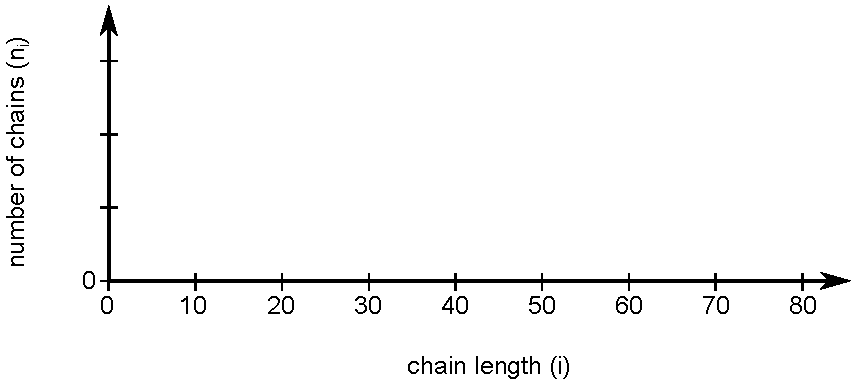
\includegraphics[width=5in]{\figpath/MWD-plots-blank}}
			}
			Example plot:
			
			\centerline{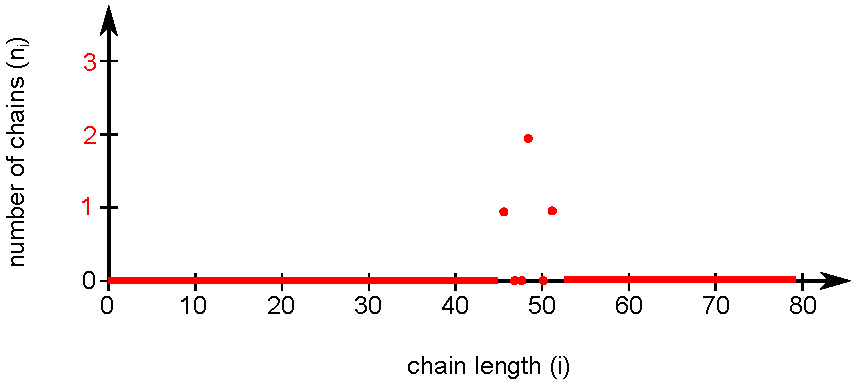
\includegraphics[width=5in]{\figpath/MWD-plots-chaingrowth-answer}}
		\end{solution}
	
	\question Calculate $M_n$, $M_w$, and \PDItext\ for this polymerization.  Assume that each bead represents a monomer with a molecular weight of 100~g/mol. \label{\labelbase:ctq:Dchain}
	
		\emph{Hint: you may find it useful use the extra columns in CTQ \ref{\labelbase:ctq:numbeadschain} to do some of the intermediate steps in the calculation, as we did in Activity 1.\ref{M-and-D}.}
	
		\begin{solution}[2.5in]{}
		
			Students should fill in the two blank columns in CTQ 1 with $n_i i$ and $n_i i^2$.  They can then calculate the sum of each column and use these sums to obtain $M_n$, $M_w$, and $\PDImath$ as in Activity 3.
			
			For the sample data shown in CTQ 1,
			
			\begin{equation*}
				M_n = M_0\frac{\sum_i i n_i}{\sum_i n_i} = (100\text{ g/mol})\frac{46\cdot 1 + 49\cdot 2 + 51\cdot 1}{1+2+1} = 4875\text{ g/mol}
			\end{equation*}
			\begin{equation*}
				M_w = M_0\frac{\sum_i i^2 n_i}{\sum_i i n_i} = (100\text{ g/mol})\frac{46^2\cdot 1 + 49^2\cdot 2 + 51^2\cdot 1}{46\cdot 1 + 49\cdot 2 + 51\cdot 1} = 4882\text{ g/mol}
			\end{equation*}
			\begin{equation*}
				\PDImath = \frac{M_w}{M_n} = \frac{4875\text{ g/mol}}{4882\text{ g/mol}} = 1.001
			\end{equation*}
		\end{solution}
	
	\question Based on your graph from CTQ \ref{\labelbase:ctq:MWDchain}, and the dispersity you calculated in CTQ \ref{\labelbase:ctq:Dchain}, would you characterize the molecular weight distribution generated by this polymerization as ``narrow'' or ``broad''?  %Briefly explain your reasoning.
	
		\begin{solution}[1in]{}
			The molecular weight distribution is narrow because there is not much variation in the chain lengths, and the dispersity is close to 1.
		\end{solution}
	
	\question If each member of your group had picked up their initiator bead at a different time, how would the molecular weight distribution and dispersity have changed?  Explain your group's reasoning in 2-3 complete sentences.
	
		\begin{solution}[1.9in]{}
			If each group member had picked up their initiator beads at different times, the molecular weight distribution would have been broader, and the dispersity would have been larger.  This is because the students who started first would have had more time to add beads to their chains and would have ended up with longer chains, while the students who started later would not have had as much time to add beads to their chains and would have ended up with shorter chains.
		\end{solution}
	
	\question If everyone in your group had picked up their initiator bead at the same time, but each person added beads at a different rate, how would the molecular weight distribution and dispersity have changed?  Explain your group's reasoning in 2-3 complete sentences.
	
		\begin{solution}[1.9in]{}
			If each group member had added beads at a different rate, the molecular weight distribution would have been broader, and the dispersity would have been larger.  This is because the students who added beads faster would end up with longer chains than in the current simulation, while students who added beads slower would end up with shorter chains.
		\end{solution}
		
\end{ctqs}

\begin{model}[Step-Growth Polymerizations]
\label{\labelbase:mdl:stepgrowth}

	Another type of polymerization uses monomers that each have two or more reactive sites.  Every molecule (monomer or polymer) may react with every other molecule (monomer or polymer) as long as they have complimentary reactive groups on their ends that are able to form a bond.
	
	Simulate this type of polymerization by doing the following:
	\begin{enumerate}
		\item Combine two bags of beads of different colors in your group's bin.  Remove any beads left over from the previous simulation if you have not done so already.
		\item Set a timer for however much time was required for the polymerization in Model \ref{\labelbase:mdl:chaingrowth}.
		\item As soon as the timer starts, start the polymerization by having each person pick up two beads \emph{of different colors}, connect them, and drop them back into the bin.
		\item Continue the polymerization by doing the following:
			\begin{itemize}
				\item Pick up two pieces (single beads, or strings of beads - try to choose as randomly as possible!) from the bin.
				\item If it is possible to connect the two pieces you picked up by connecting beads \emph{of different colors}, connect the two pieces and return them to the bin.
				\item Otherwise, return both pieces to the bin and try again.
			\end{itemize}
		\item Continue connecting beads until your timer goes off.
	\end{enumerate}
	
	Use the chains generated in this simulation to answer this Model's CTQs, below.

\end{model}
	
\begin{ctqs}

	\question Count the number of beads in each chain, and fill in the following table.  Count unreacted monomer beads as chains of length 1. \label{\labelbase:ctq:numbeadsstep}
		
		\begin{center}
		\renewcommand{\arraystretch}{2}
			\begin{tabular}{|c|c|c|c|}
				\hline
				\textbf{Chain Length ($i$)} & \textbf{Number of Chains of Length $i$  ($n_i$)} & \hspace{0.75in} & \hspace{0.75in} \\\hline
				\answer{1}&\answer{58}&&\\\hline
				\answer{2}&\answer{45}&&\\\hline
				\answer{3}&\answer{29}&&\\\hline
				\answer{4}&\answer{24}&&\\\hline
				\answer{5}&\answer{12}&&\\\hline
				\answer{6}&\answer{13}&&\\\hline
				\answer{8}&\answer{3}&&\\\hline
				\answer{9}&\answer{5}&&\\\hline
				\answer{10}&\answer{2}&&\\\hline
				\answer{15}&\answer{1}&&\\\hline
				&&&\\\hline
				&&&\\\hline
				&&&\\\hline
				&\answer{(sample data - student answers will vary)}&&\\\hline
				&&&\\\hline
				&&&\\\hline
			\end{tabular}
		\end{center}
		
	\question Sketch a graph of $n_i$ vs $i$ and briefly describe its shape. \label{\labelbase:ctq:MWDstep}
	
		\begin{solution}[3in]{%
			\centerline{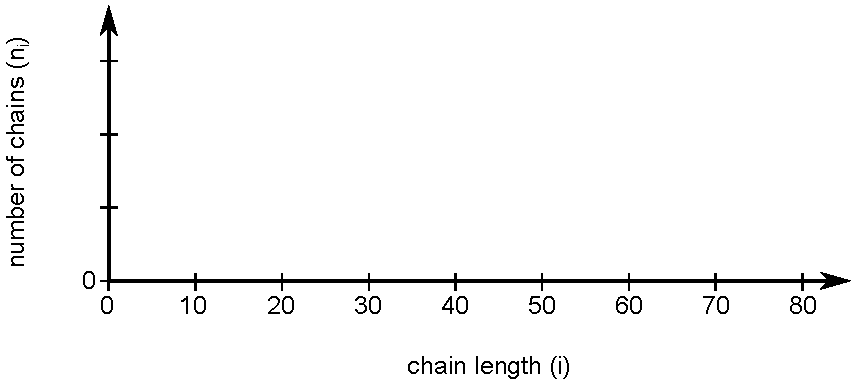
\includegraphics[width=5in]{\figpath/MWD-plots-blank}}
			}
			Example plot:
			
			\centerline{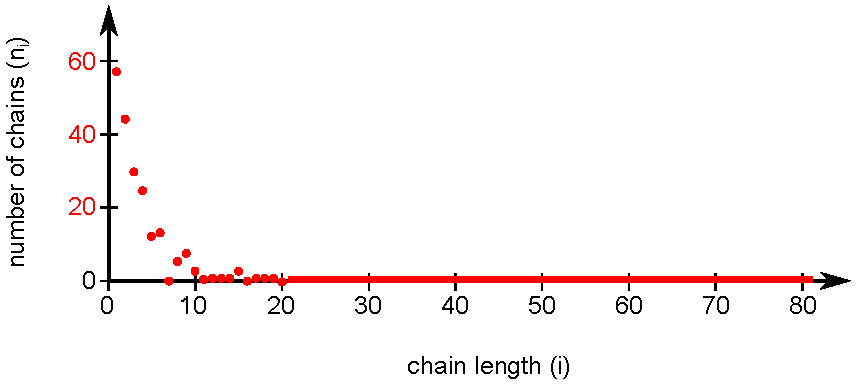
\includegraphics[width=5in]{\figpath/MWD-plots-stepgrowth-answer}}
		\end{solution}
	
	\question Calculate $M_n$, $M_w$, and \PDItext\ for this polymerization.  Assume that each bead represents a monomer with a molecular weight of 100~g/mol. \label{\labelbase:ctq:Dstep}
	
		\begin{solution}[3in]{}
			This calculation follows the same approach as in CTQ \ref{\labelbase:ctq:Dchain}.
			
			For the sample data shown above,
			\begin{align*}
				\sum_i n_i = 192 && \sum_i i n_i = 573 && \sum_i i^2 n_i = 2673
			\end{align*}
			so
			\begin{align*}
				M_n = 298\text{ g/mol} && M_w = 466\text{ g/mol} && \PDImath = 1.56
			\end{align*}
			
			(Note that the dispersity is somewhat lower than the limiting value of 2 for step-growth polymerizations because the extent of reaction is relatively low.)
		\end{solution}
	
	\question Based on your graph from CTQ \ref{\labelbase:ctq:MWDstep}, and the dispersity you calculated in CTQ \ref{\labelbase:ctq:Dstep}, would you characterize the molecular weight distribution generated by this polymerization as ``narrow'' or ``broad''?  %Briefly explain your reasoning.
	
		\begin{solution}[1in]{}
			This molecular weight distribution is not extremely broad (the dispersity is not larger than 2), but it is also not nearly as narrow as the molecular weight distribution generated in Model \ref{\labelbase:mdl:chaingrowth}.  A dispersity of 1.5 is right on the edge of what we typically consider narrow.
		\end{solution}
	
	\question Suppose you had kept going with the simulation until no more  connections could be made.  What would be the result?  Explain your group's reasoning in 2-3 complete sentences.
	
		\begin{solution}[1.75in]{}
			Eventually, all of the beads would have ended up connected into a single long chain.
		\end{solution}
	
	\question If there had been significantly more beads of one color than the other, how would the final distributions of chains be different?  Explain your group's reasoning in 2-3 complete sentences.
	
		\begin{solution}[2in]{}
			If there were significantly more beads of one color than the other, the final sample would contain many shorter chains, each capped by the color of bead present in excess.  This is because once all of the chains end in the color present in excess, no further reactions can take place, so the chains stop growing.
		\end{solution}
	
\end{ctqs}

\begin{infobox}
	The type of polymerization you simulated in Model  \ref{\labelbase:mdl:chaingrowth} is called a \emph{chain-growth} polymerization, while the type of polymerization you simulated in Model  \ref{\labelbase:mdl:stepgrowth} is called a \emph{step-growth} polymerization.
	
	All of the polymerization methods we discuss in class will fall into one of these two categories, and it is useful to recognize the advantages and disadvantages of each approach.
\end{infobox}

\begin{ctqs}
	\question Which polymerization mechanism (chain-growth or step-growth) gave longer polymers in the time allowed for the simulation?
	
		\begin{solution}[1in]{}
			The chain-growth polymerization gave longer polymers in the time allowed for the simulation.
		\end{solution}
	
	\question Which method would give the longest polymers if there were an infinite amount of time?  Explain your group's reasoning in 1-2 complete sentences.
	
		\begin{solution}[1.75in]{}
			If there were an infinite amount of time, the step-growth polymerization would give longer chains because the monomers could (if there were equal numbers of beads of each color) theoretically all combine into a single long chain, while the monomers for the chain-growth polymerization are necessarily divided up into a number of chains equal to the number of initiator beads.
		\end{solution}
	
	\question Which polymerization mechanism gave a larger dispersity?  In 2-3 complete sentences, explain why your group thinks this happened.
	
		\begin{solution}[1.75in]{}
			The step-growth polymerization gave a larger dispersity.  This is because the polymerization process was much more random, and so there ended up being a broader distribution of chain lengths.
		\end{solution}
	
	\question If you needed to make a batch of 700~kg/mol polyethylene, which type of polymerization would you choose?  Explain your group's choice in 1-2 complete sentences.
	
		\begin{solution}[1.75in]{}
			A chain-growth polymerization would be most suitable.  Although step-growth polymerizations can theoretically reach higher molecular weights, they take a VERY long time to get there, so it would likely be impractical to prepare a 700~kg/mol polymer using this method.
			
			(Note: once students learn about the chemistries for chain-growth and step-growth polymerization, they will hopefully also recognize that polyethylene can't be prepared by step-growth polymerization, either, because the ethylene monomers can't react directly with each other.)
		\end{solution}
	
\end{ctqs}

\clearpage
\begin{exercises}

		\exercise In a brief paragraph, describe the key differences between the chain-growth and step-growth polymerization mechanisms.
		
		\begin{solution}{}
			In chain-growth polymerizations, the monomers can only react with the ``active'' end of a polymer chain, while in a step-growth polymerization, they can react directly with each other or with other chains.  The kinetics are also very different: chain growth polymerizations generate longer chains much more quickly than step-growth polymerizations do.  Finally, the molecular weight distributions are different. At least for the chain-growth process demonstrated in this activity (which, following the simulation instructions, is essentially an ideal living chain-growth polymerization), the molecular weight distribution was sharply peaked at a relatively long chain length, while for the step-growth polymerization the molecular weight distribution was much broader and centered around shorter chain lengths (and, in fact, the most common species in the mixture was unreacted monomer, or chains of length 1!).
		\end{solution}
		
		\exercise Summarize the key conditions necessary for a chain-growth polymerization to achieve a narrow molecular weight distribution.
		
			\begin{solution}{}
				As demonstrated in this activity, two of the key conditions necessary for a chain-growth polymerization to achieve a narrow molecular weight distribution are:
				\begin{itemize}
					\item All chains must start growing at the same time
					\item All chains must grow at the same rate
				\end{itemize}
				
				Although not demonstrated in this activity, two additional requirements apply:
				\begin{itemize}
					\item The polymerization must proceed in the absence of irreversible termination reactions
					\item The polymerization must proceed in the absence of irreversible chain-transfer reactions
				\end{itemize}
				These requirements will be covered in more detail later in this course.
			\end{solution}
			
\end{exercises}
	
\end{activity}